\documentclass[UTF8, xcolor=table]{beamer}
\usepackage[BoldFont,SlantFont]{xeCJK}
\setCJKmainfont[BoldFont={Adobe Heiti Std},ItalicFont={Adobe Kaiti Std}]{AdobeSongStd-Light}
% \setCJKmainfont[BoldFont={Adobe Heiti Std},ItalicFont={Adobe Kaiti Std}]{SimSum} %Windows先编译使用这个字体

\usepackage{latexsym,amssymb,amsmath,amsbsy,amsopn,amstext,xcolor,multicol}
\usepackage{graphicx,wrapfig,fancybox}
\usepackage{pgf,pgfarrows,pgfnodes,pgfautomata,pgfheaps,pgfshade}
\usepackage{thubeamer}
\usepackage[backend=bibtex,sorting=none]{biblatex} % [参考文献格式](https://www.sharelatex.com/blog/2013/07/31/getting-started-with-biblatex.html) %mac IEEE not found
\usepackage{array}
\usepackage{bm}
\usepackage{caption}
\RequirePackage[font=footnotesize]{subcaption}
\usepackage{multirow}
\usepackage{booktabs}
\usepackage{tikz}
\usepackage{tikzscale}
\usepackage{animate}

\defbibheading{bibliography}[\bibname]{} %avoid printbibliography 自动生成目录
\addbibresource{../main.bib}
\setbeamertemplate{bibliography item}[text] 

\usepackage{boxedminipage} %for: bvh border
\def\fourgraphicswidth{0.35} %0.3\textwidth

\usepackage{algorithm} %%format of the algorithm
\usepackage{algpseudocode}
\floatname{algorithm}{算法}
\renewcommand{\algorithmicrequire}{\textbf{输入:}} % Use Input in the format of Algorithm
\renewcommand{\algorithmicensure}{\textbf{输出:}} % UseOutput in the format of Algorithm
\algrenewcommand{\algorithmiccomment}[1]{ $//$ #1}

\usepackage{listings}
\renewcommand\lstlistingname{代码}
\renewcommand\lstlistlistingname{代码}

\lstset{framexleftmargin=1.4em,
        xleftmargin=1.8em,
        basicstyle=\ttfamily\small,
        %frame=shadowbox, numberstyle=\tiny, breaklines=true,
        frame=single,
        numberstyle=\tiny, breaklines=true,
        keywordstyle=\color{blue!70}\bfseries,
        %commentstyle=\color{red!50!green!50!blue!50},
        rulesepcolor=\color{red!20!green!20!blue!20},
        numbers=none,fontadjust=true}
\lstdefinelanguage{shader}{morekeywords={uniform, layout, uniform, vec2, vec3, vec4, in, out, gl_Position, dot, flat, int ,float, gl_VertexID, xyz, w, x, y, z, location, version, sampler2DRect, bgr, gl_FragData, texture2DRect, gl_TexCoord,for,xy},morecomment=[l]{//}}

\begin{document}

\setbeamerfont{footnote}{size=\tiny}
\setbeamerfont{caption}{size=\scriptsize}
\setbeamertemplate{caption}[numbered]
\setbeamerfont{subsection in toc}{size=\footnotesize}
\renewcommand*{\bibfont}{\footnotesize}

\graphicspath{{../}}

\title[融合长短记忆神经网络与卷积特征学习的图像语义分割]{中山大学本科毕业论文演示文稿非正式模版}
\author[陈冠英]{}%{(申请中山大学工学学士学位论文答辩报告)\\ \vskip 20pt 学~~~~~~生:陈~冠~英}
\institute[中山大学~电子信息与工程学院~\&~自动化]{}%{\small \vskip 38pt 电子信息与工程学院~自动化}
\date{} %{\small \vskip -17pt二〇一六年五月}

%% make title %%
\frame{
	\titlepage
	\vspace{-23mm}
	\begin{figure}[h]
		\centering
		\includegraphics[width=\textwidth]{image/illustration/networkstructure.pdf}
	\end{figure}
}

\frame {
	\frametitle{目录}
	%\begin{multicols}{2}
	\tableofcontents[sections={<1-7>}]
}

%%
% 引言或背景
% 引言是论文正文的开端,应包括毕业论文选题的背景、目的和意义;对国内外研究现状和相关领域中已有的研究成果的简要评述;介绍本项研究工作研究设想、研究方法或实验设计、理论依据或实验基础;涉及范围和预期结果等。要求言简意赅,注意不要与摘要雷同或成为摘要的注解。
% modifier: 黄俊杰(huangjj27, 349373001dc@gmail.com)
% update date: 2017-04-15
%%

\chapter{引言}
%定义,过去的研究和现在的研究,意义,与图像分割的不同,going deeper
\label{cha:introduction}
\section{问题介绍}
多维尺度变换是一种将高维多元数据在低维空间中可视化的方法。多维尺度变换的目标是将原始数据降维到一个低维空间,并试图使低维空间中由降维产生的形变最小。一般可以将多维尺度变换解决的问题描述为:当$n$个对象之间的距离或相似性已知时,寻求这些对象在给定维数的低维空间中的表示,并使低维空间中对象间的距离与相似性与最开始给定的相似。例如,一个形象的例子:假设你有一张地图,上面有$n$个城市。通常这样的地图上会给出城市之间的距离。此时MDS所想解决的问题就是,如果只给出了城市两两之间的距离信息,能否尽可能重构出原来的地图。MDS根据涉及的对象是否可以计量分为度量型多维尺度变换(Metric MDS)和非度量型多维尺度变换(Non-metric MDS)。在度量型多维尺度变换中,又将距离度量为欧式距离的称为经典多维尺度变换(Classical MDS, CMDS)。

\section{主要内容}
本文试图解决的问题是,当已知$n$个点两两之间部分的距离信息时,能否在尽量保持距离信息的前提下,重构出三维空间中这$n$个点的坐标。显然,如果距离信息完整或者缺失比率比较少的时候,经典多维尺度变换的方法能比较有效的解决这个问题。但当距离信息缺失比例比较大的情况下,经典多维尺度变换的方法的效果就不算很好。因此,本文中介绍了一种更有效的方法,SMACOF。SMACOF试图最小化重构空间点与点之间的距离与原距离信息之间的平方误差。同时引入了一个权重变量,允许输入的给定距离信息中有缺失值,并称这个平方误差为Stress Function。最小化Stress Function的方法有很多,如Krustal\cite{kruskal1964multidimensional}的用迭代最速下降的方法来求Stress Function的最小值。Jan de Leeuw\cite{de2011applications}的SMACOF方法采用iterative majorization的方法,是一种收敛效果更好的算法。
除了上述两种经典的MDS算法之外,受经典多维尺度变换方法还有距离平方矩阵秩的性质的启发,我们考虑先通过低秩矩阵恢复的方法恢复距离矩阵信息,再使用经典多维尺度变换的方法重构出坐标。近几年解决低秩矩阵填充问题的方法有很多,如APG\cite{toh2010accelerated}(Accelerated Proximal Gradient),FPCA\cite{ma2011fixed}(Fixed Point Continuation with Approxiamte SVD),ADMIRA\cite{lee2010admira}(Atomic Decomposition for Minimum Rank Approximation)等。
本文后半部分主要介绍了两种低秩矩阵的恢复算法SVT(Singular Value Thresholding)\cite{cai2010singular}和OPTSPACE\cite{keshavan2010matrix}。尝试先使用上述两种低秩矩阵恢复的方法恢复距离信息,再使用经典多维尺度变换技术来重构坐标。最后,我们对前述算法进行数值实验,给出各算法在球面($S^2$)和牛形曲面($Cow$)两个数据集上的数值实验结果,从直观恢复结果,Error指标以及算法收敛速度三个方面来比较各算法分别在两个数据集的效果,并尝试从数据集和算法特点来分析产生效果差别的原因。

\section{本文结构与章节安排}
本文的剩余部分的结构大致如下。第 \ref{cha:classMDS}章中,我们将介绍经典多维尺度变换的背景理论和具体算法。第
\ref{cha:SMACOF}章中,我们首先介绍Majorization方法,引入Majorizing Function还有Stress Function的概念。并最后用Majorization的方法来最小化Stress function,得到最终的SMACOF算法。第 \ref{cha:SVT}章和第 \ref{cha:OPTSPACE}章中,首先介绍了距离平方矩阵秩的性质,接下来介绍SVT和OPTSPACE两种低秩矩阵恢复的方法,并在原始OPTSPACE算法的基础上引出在特殊情况下有更好效果的Incremental OPTSPACE算法。最后,在第 \ref{cha:numerical}章中,我们给出了具体的数值实验和分析过程,以及最终的分析比较的结果。
\section{深度神经网络}
\frame
{
  \frametitle{\secname~ }
  \begin{block}{前馈神经网络}
	  传统的人工神经网络
  \end{block}
  \begin{block}{卷积神经网络}
	  目前最为流行的,广泛应用于视觉任务的神经网络
  \end{block}
  \begin{block}{长短记忆网络}
	  与卷积网络相比,更适用于处理时序信号
  \end{block}
}
\subsection*{深度神经网络}
\frame{
	\frametitle{前馈神经网络结构}
    \begin{columns}[onlytextwidth]
		\begin{column}{0.5\textwidth}
			\vspace{-1.5em}
		\begin{itemize}
			\item 有向无环图的结构
			\item 输入层(数据特征)
			\item 隐含层(映射后的特征)
			\item 输出层(预测结果)
			\item 反向传播算法(训练方法)
		\end{itemize}
		\end{column}
		\begin{column}{0.5\textwidth}
		\begin{figure}[h] %structure of LSTM
			\centering
			\includegraphics[width=0.9\textwidth]{image/illustration/network1.pdf}
			\caption{前馈神经网络模型示意图}
			\label{fig:lstm}
		\end{figure}
		\end{column} 
	\end{columns}
}

\frame{
   \frametitle{卷积神经网络}
   \vspace{-0.8em}
	\begin{figure}
		\centering
		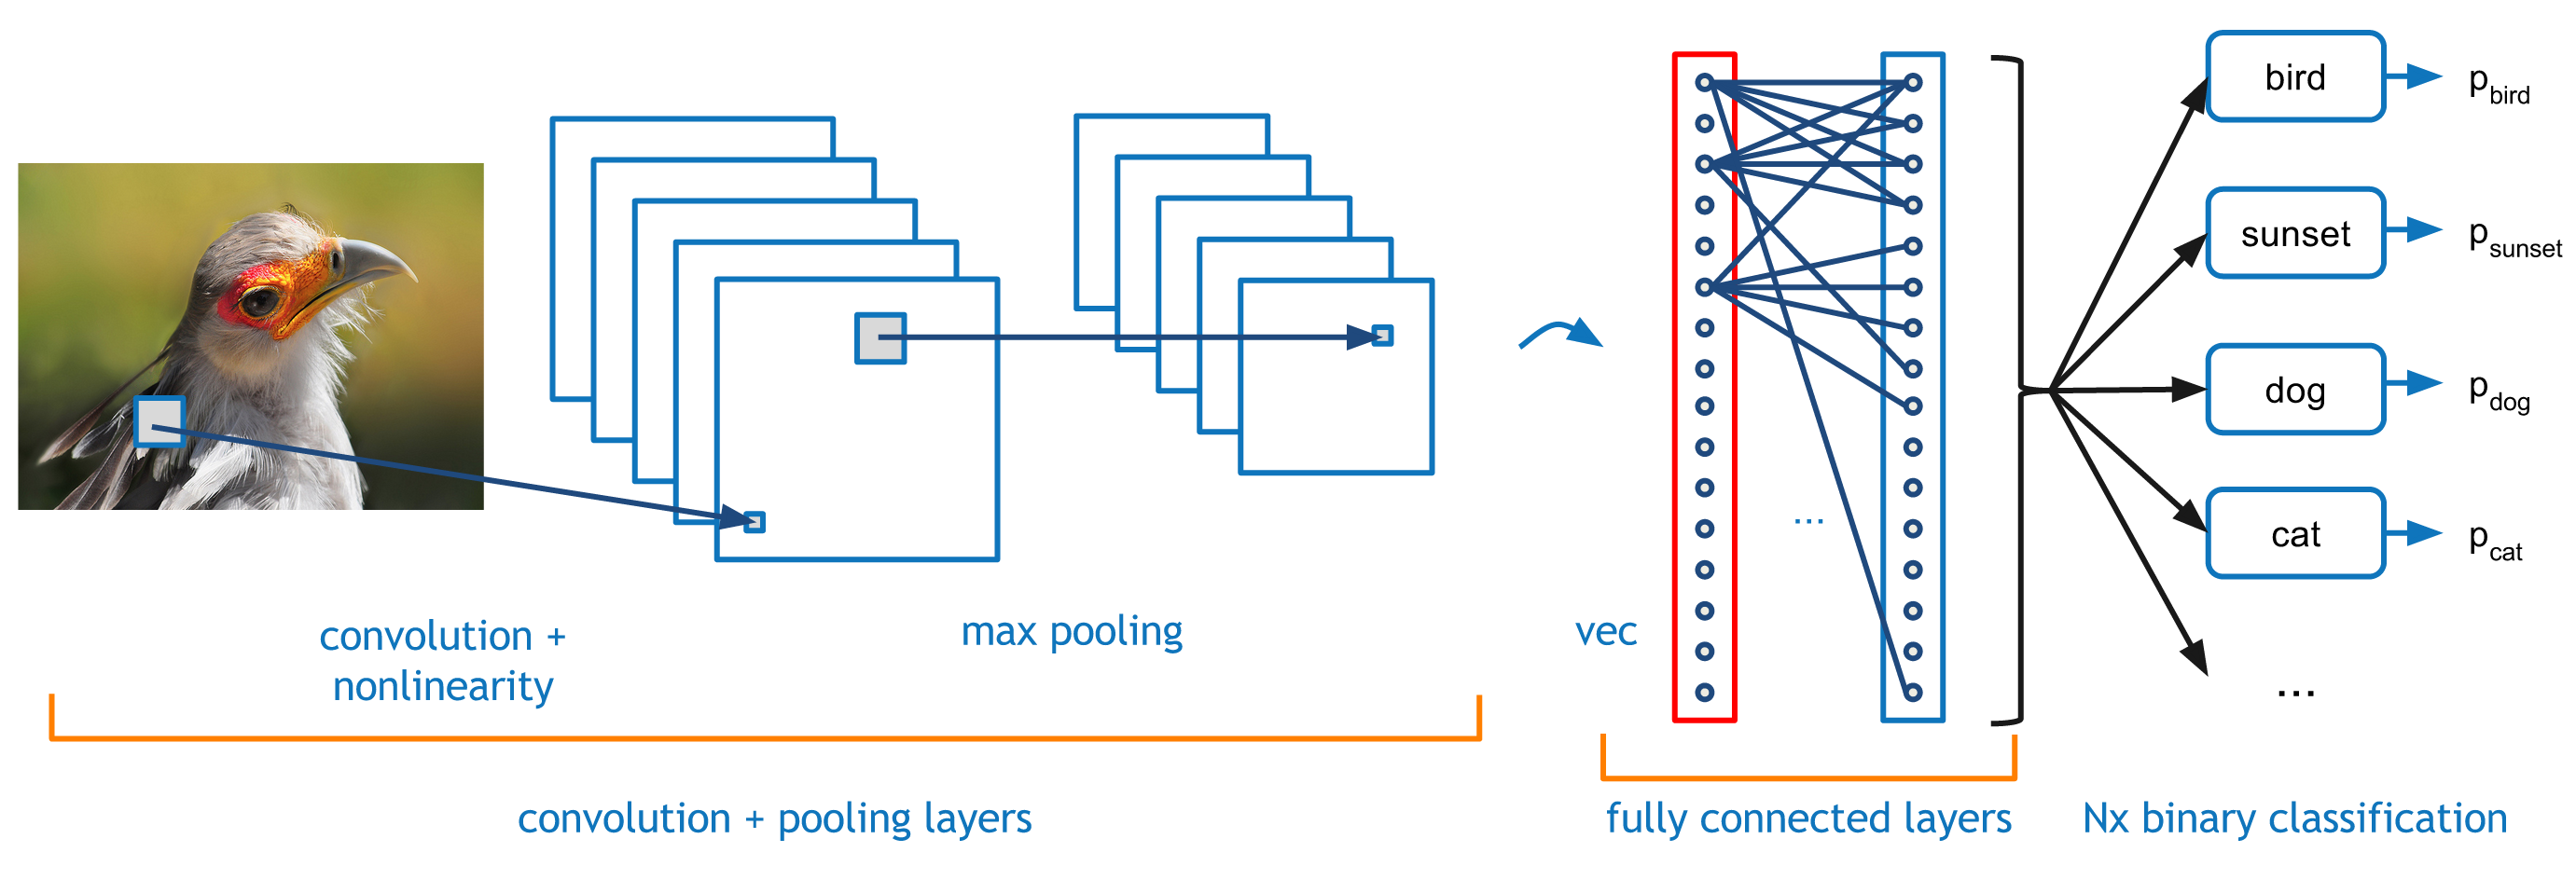
\includegraphics[width=0.8\textwidth]{figures/CNN}
		\caption{卷积网络模型示意图}
		\label{fig:network1}
	\end{figure}  
   \vspace{-0.8em}
	\begin{block}{与前馈神经网络的区别}
	\begin{itemize}
		\item 直接作用于二维图像,无需特征设计阶段
		\item 卷积层,池化层
		\item 局部感知域,权重共享
	\end{itemize}
	\end{block}
}

\frame{
	\frametitle{长短记忆网络(处理一维信号)}
	\tiny
	\vspace{-2em}
    \begin{columns}[onlytextwidth]
        \begin{column}{0.5\textwidth}
	    \begin{figure}[h] %structure of LSTM
	    	\centering
	    	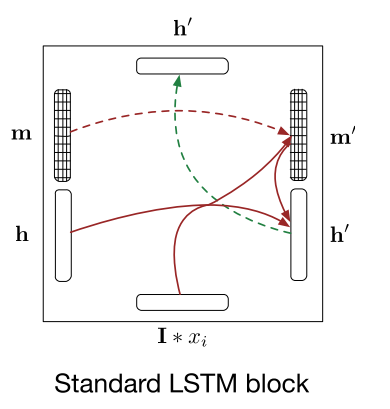
\includegraphics[width=0.6\textwidth]{figures/lstmblock1}
	    	\caption{长短记忆网络区块示意图}
	    	\label{fig:lstm}
	    \end{figure}
		\end{column} 
		%%%%%%% new column
		\begin{column}{0.5\textwidth}
			\begin{boxedminipage}{0.8\textwidth}
			\vspace{-1.5em}
			\begin{align}
				\label{eq:lstm}
				\begin{split}
				\textbf{g}^u &= \delta(\textbf{W}^u*\textbf{H}) \\
				\textbf{g}^f &= \delta(\textbf{W}^f*\textbf{H}) \\
				\textbf{g}^o &= \delta(\textbf{W}^o*\textbf{H}) \\
				\textbf{g}^c &= \mbox{tanh}(\textbf{W}^c*\textbf{H}) \\
				\textbf{m}' &= \textbf{g}^f \odot \textbf{m} + \textbf{g}^u \odot \textbf{g}^c \\
				\textbf{h}' &= \mbox{tanh}(\bf{g}^o \odot \bf{m}') \\
					\textbf{H} & = \begin{bmatrix}
					I*\textbf{x}_i \\ \textbf{h}
					\end{bmatrix}
			\end{split}
			\end{align}
		\end{boxedminipage}
		\end{column}
    \end{columns}
	
	\vspace{-1em}
	\begin{block}{缩写形式}
	\footnotesize
	\begin{equation*}
		(\textbf{h}', \textbf{m}') = \mbox{LSTM}\bigr(\textbf{H},\textbf{m},\textbf{W} \bigr)
	\end{equation*}
	其中\textbf{W}包含了四个门权值矩阵$\textbf{W}^u,\textbf{W}^f,\textbf{W}^o,\textbf{W}^c$。
	\end{block}
}

\frame{
	\frametitle{网格型长短记忆网络(处理N维信号)}
	\vspace{-1.5em}
	\begin{figure}[h]
	\centering
		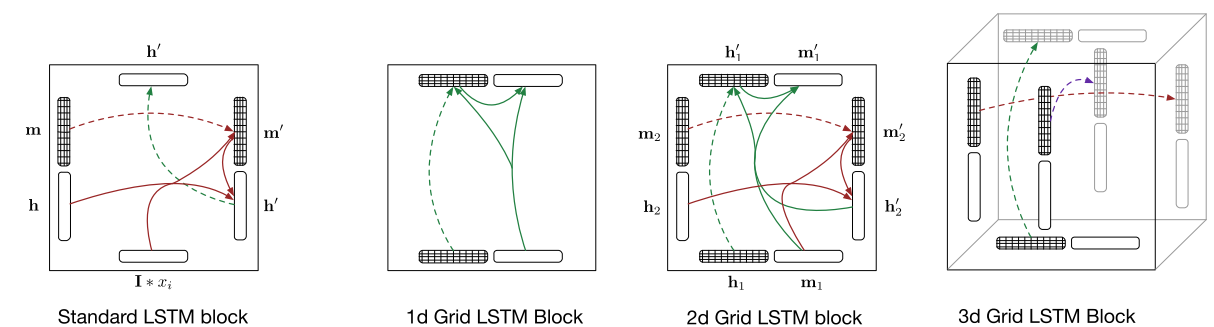
\includegraphics[width=\textwidth]{figures/gridlstm}
		\caption{网格型长短记忆网络区块示意图[Kalchbrenner et al, Grid LSTM, ICLR 2016]}
	\end{figure}
	\vspace{-2em}
	\begin{block}{网格型长短记忆网络更新过程}
	\tiny
	\begin{columns}[onlytextwidth]
		\begin{column}{0.4\textwidth}
		\vspace{-0.5em}
			\begin{equation}
				\textbf{H} = \begin{bmatrix}
					\textbf{h}_i \\ \vdots \\ \textbf{h}_N
				\end{bmatrix}
			\end{equation}
		\end{column}
		\begin{column}{0.6\textwidth}
		\vspace{-1em}
			\begin{align}
				\begin{split}
				(\textbf{h}_1', \textbf{m}_1') & =  \mbox{LSTM}(\textbf{H}, \textbf{m}_1, \textbf{W}_1) \\ &\mbox{ }\vdots \\
				(\textbf{h}_N', \textbf{m}_N') & =  \mbox{LSTM}(\textbf{H}, \textbf{m}_N, \textbf{W}_N)
				\end{split}
				\label{eq:gridlstm}
			\end{align}
		\end{column}
	\end{columns}
	\end{block}
}
\endinput

\section{网络模型结构}
\subsection*{网络模型结构}
\frame{
  \frametitle{网络整体结构}
	\begin{figure}[h]
		\centering
		\includegraphics[width=0.9\textwidth,height=0.28\textwidth]{image/illustration/networkstructure.pdf}
		\caption{网络整体结构图}
		\label{fig:networkstructure}
	\end{figure}
	\vspace{-1em}
	\small
	\begin{block}{}
	\begin{itemize}
		\item  四个组成部分:\textbf{卷积网络部分},过渡层,\textbf{网格型长短记忆网络部分},前向卷积层
		\item 核心思想:在卷积网络后堆叠多层网格型长短记忆层
	\end{itemize}
	\end{block}
}
\frame{
	\frametitle{卷积网络部分}
	\vspace{-1em}
	\footnotesize
	\begin{block}{}
	\begin{itemize}
		\item 基于$VGG_{16}$模型\footnote{Simonyan \& Zissermanet, Very deep Convolutional Networks For Large-scale Image Recognition, ICLR 2015}, 含有16层卷积层
		\item 使用了“孔算法”,在不损失精度的情况下将模型参数减少了 6.5 倍\footnote{Chen et al, DeepLab-LargeFOV, ICLR 2015}
	\end{itemize}
	\end{block}
	\vspace{-1em}
	\begin{figure}[h]
		\centering
		\includegraphics[width=0.7\textwidth]{image/illustration/hole.pdf}
		\caption{"孔算法"示意图}
	\end{figure}
}

\frame{
\frametitle{网格型长短记忆网络部分}
	\vspace{-1em}
    \begin{columns}%[onlytextwidth]
        \begin{column}{0.6\textwidth}
        \vspace{0.2em}
		\begin{figure}
			\centering
			\includegraphics[width=\textwidth]{image/illustration/neighboring.pdf}
			\caption{九维网格型长短记忆网络层之间的通信示意图}
			\label{fig:neighboring}
		\end{figure}
		\end{column} 
		%%%%%%% new column
		\begin{column}{0.5\textwidth}
			\footnotesize
			\vspace{-1.5em}
			\begin{align}
				\begin{split}
				(\hat{\textbf{h}}_{i,j}^0,\hat{\textbf{m}}_{i,j}^0) &= \mbox{LSTM}(\textbf{H}_{i,j},\textbf{m}_{i,j}^0,\textbf{W}_i) \\
				(\hat{\textbf{h}}_{i,j}^1,\hat{\textbf{m}}_{i,j}^1) &= \mbox{LSTM}(\textbf{H}_{i,j},\textbf{m}_{i,j}^1,\textbf{W}_i) \\
				\vdots \\
				(\hat{\textbf{h}}_{i,j}^N,\hat{\textbf{m}}_{i,j}^N) &= \mbox{LSTM}(\textbf{H}_{i,j},\textbf{m}_{i,j}^N,\textbf{W}_i) \\
				\textbf{H}_{i,j} &= [\textbf{h}_{i,j}^0\mbox{ }\textbf{h}_{i,j}^1\mbox{ }...\mbox{ }\textbf{h}_{i,j}^N]^T
				\end{split}
			\end{align}
		\end{column}
    \end{columns}
	\footnotesize
	\vspace{-1em}
	\begin{block}{九维网格型长短记忆网络}
		\vspace{-0.7em}
		\begin{itemize}
			\item 每个位置的预测会受到上一层相邻八邻域特征的影响
			\item 随着层数的堆叠,每一位置将会有更大的感知域。
			\item 网格型长短记忆网络的层数通过实验来确定
		\end{itemize}
	\end{block}
}



\chapter{SVT}
\label{cha:SVT}
\section{介绍}
接下来我们所需要解决的问题可描述为:根据一小部分已知的元素,重构或者恢复一个$n\times n$低秩矩阵$\mathbf{M}$。精确矩阵填充问题(exact matrix completion problem)等价于找到一个秩最小的矩阵与已知的矩阵元素相对应。即:
\begin{align}
\label{al: rank}
&\min \ rank(\mathbf{X}) \nonumber\\
s.t.\ &\mathbf{X}_{ij} = \mathbf{M}_{ij}, (i,j)\in \Omega
\end{align}
这是一个NP-Hard问题,在压缩感知(compressed sensing)领域中,一个核心的问题就是找到满足一系列限制条件的最稀疏的向量。即:
\begin{align*}
&\min \ \left\|x\right\|_{l_0}\\
s.t.\ &Ax = b,
\end{align*}
其中$l_0$范数表示向量的稀疏性,即向量中非零元素的个数。为了解决这个问题,一个通用的方法是解决下面的优化问题:
\begin{align*}
&\min \ \left\|x\right\|_{l_1}\\
s.t.\ & Ax = b,
\end{align*}
其中$l_1$范数是向量中所有元素绝对值之和。$l_1$范数的优化问题,在适当的条件下可以提供原$l_0$问题的最优解。现在回到原来的优化问题(\ref{al: rank}),秩可以视为矩阵非零奇异值的个数,而核范数是矩阵所有奇异值之和。故可以将矩阵$rank(\cdot)$类比成向量的$l_0$范数,矩阵的核范数$\|\cdot\|_*$可以对应成$l_1$范数。矩阵秩的优化问题和压缩感知问题之间的联系在\cite{recht2010guaranteed}中有详细的研究。由上述想法Candes and Recht将(\ref{al: rank})中的问题凸松弛化为核范数的优化问题,即最小化奇异值的和\cite{candes2009exact}。如下:
\begin{align}
\label{al:optimize}
&\min \ \left\|\mathbf{X}\right\|_* , \nonumber\\
s.t.\ &\mathbf{X}_{ij} = \mathbf{M}_{ij}, (i,j)\in \Omega
\end{align}
同时\cite{candes2009exact}中证明了,对于一个$m\times n$秩为$r$的矩阵$\mathbf{M}$,当已知元素个数$|\Omega|$满足,$|\Omega|\geq C(\alpha) r n^{1.2}log(n)$,且满足incoherence的性质时,解决问题(\ref{al:optimize})可以很大概率的恢复矩阵$\mathbf{M}$。

SVT就为解决问题(\ref{al:optimize})的方法之一。 同时相较于\cite{liu2009interior}中的interior point方法, SVT更能解决数据量比较大的情况下的问题。SVT算法是一种迭代算法,产生一个矩阵序列$\{\mathbf{X}^k,\mathbf{Y}^k\}$。每一步的迭代操作主要就是对矩阵$\mathbf{Y}^k$的奇异值进行一个软阈值操作(soft-thresholding operation)。由于$\mathbf{Y}^k$为一稀疏矩阵,SVT算法有每一次迭代中计算代价低,存储空间要求低的优点。


\section{距离平方矩阵的低秩性}
与前面的定义相同,$\mathbf{X} = [\mathbf{x}_1, \dots, \mathbf{x}_n]$, $\mathbf{x}_i \in \mathbb{R}^p$,并假设$p\ll n$,$\mathbf{D}$为距离平方矩阵。\cite{dokmanic2015euclidean}中提出了距离平方矩阵的秩应满足的性质,我们将它叙述成定理并给出相应证明如下:
\begin{theorem}
$rank(\mathbf{D}) \leq (p+2)$
\end{theorem}

\begin{proof}
由
\begin{equation*}
    D = \mathbf{1} \cdot diag(\mathbf{X}^\intercal\mathbf{X})^\intercal + diag(\mathbf{X}^\intercal\mathbf{X}) \cdot \mathbf{1}^\intercal - 2 \mathbf{X}^\intercal\mathbf{X}
\end{equation*}

由$rank(\mathbf{X})\leq p$, 则$rank(\mathbf{X}^\intercal\mathbf{X}) \leq p$。又上式中的其他两项的秩均为$1$,由秩的性质知
\begin{equation*}
\begin{split}
    rank(\mathbf{D}) &\leq rank(\mathbf{1} \cdot diag(\mathbf{X}^\intercal \mathbf{X})) + rank(diag(\mathbf{X}^\intercal\mathbf{X}) \cdot \mathbf{1}^\intercal) - rank(2\mathbf{X}^\intercal\mathbf{X})\\
    &\leq p + 2
\end{split}
\end{equation*}
\end{proof}
故由上定理可知距离平方矩阵的秩最大只能为$(p + 2)$,故当$d\ll n$时,$rank(\mathbf{D})\ll n$。故接下来试图采用低秩矩阵的恢复方法来恢复距离平方矩阵。

\section{SVT算法}
在本小节将介绍\cite{cai2010singular}中的SVT算法来解决(\ref{al:optimize})中的优化问题,首先定义一个正交算子$P_{\Omega}$
$$
P_{\Omega}(\mathbf{M})_{ij} = \left\{\begin{array}{cc}
     \mathbf{M}_{ij} & (i,j) \in\Omega \\
     0 & otherwise
\end{array}
$$
故优化问题可写成
\begin{align}
\label{al: ortho}
&\min \ \left\|\mathbf{X}\right\|_*\nonumber\\
s.t.\ & P_{\Omega}(\mathbf{M}) = P_{\Omega}(\mathbf{X})
\end{align}
依照\cite{cai2010singular}中,对于给定的软阈值$\tau$和步长序列$\{\delta_k\}$,初值$\mathbf{Y}_0$,有迭代算法:
$$
\left\{\begin{array}{cc}
\label{arr: iter}
     \mathbf{X}^k &= \mathbf{D}_\tau(\mathbf{Y}^{k-1}) \nonumber\\
     \mathbf{Y}^k &= \mathbf{Y}^{k-1} + \delta_kP_\Omega(\mathbf{M} - \mathbf{X}^k)
\end{array}\right
$$
其中$D_{\tau}$为Shrinkage operator。若$\mathbf{X}\in\mathbb{R}^{n_1\times n_2}, rank(\mathbf{X}) = r$,记$\mathbf{X}$的奇异值分解为$\mathbf{X = U}\Sigma \mathbf{V}^\intercal, \Sigma = diag\left(\{\sigma_i\}_{1\leq i \leq r}\right), \mathbf{U}\in\mathbb{R}^{n_1\times r}, \mathbf{V}\in \mathbb{R}^{n_2\times r}$
则
\begin{equation*}
\mathbf{D}_\tau(\mathbf{X}) = \mathbf{U}\mathbf{D}_\tau(\Sigma)\mathbf{V}^\intercal, 
\mathbf{D}_\tau(\Sigma) = diag(\{\sigma_i - \tau\}_+)
\end{equation*}

在\cite{cai2010singular}中已经证明$\{ \mathbf{X}^k\}$序列收敛到如下优化问题的解
\begin{align*}
&\min \ \tau\left\|\mathbf{X}\right\|_* + \frac{1}{2}\left\|\mathbf{X}\right\|_F^2  \\
s.t.\ & P_{\Omega}(\mathbf{M}) = P_{\Omega}(\mathbf{X})
\end{align*}
而当$\tau \to \inf$时,上述优化问题即逼近(\ref{al: ortho})式的解。
由\cite{cai2010singular}中已经证明,当步长$\delta$大于0,小于2时的时候,该算法一定收敛,但是收敛速度会很慢。故采用论文中建议的数值,即若$|\Omega|=m$,则$\delta = 1.2\frac{n_1n_2}{m}$。

关于$\mathbf{Y}^0$初值的选择,记$k_0$为满足如下条件的整数
\begin{equation*}
    \frac{\tau}{\delta\|P_\Omega(\mathbf{M})\|_2}\in (k_0-1, k_0].
\end{equation*}
由于$\mathbf{Y}^0 = \mathbf{0}$,根据前面的迭代算法可以看出,$\mathbf{X}^k = \mathbf{0}$且$\mathbf{Y}^k = k\delta P_{\Omega}(\mathbf{M})$,$k = 1,\dots,k_0$。故可以跳过计算$\mathbf{X}^1,\dots,\mathbf{X}^{k_0}$的过程,直接以$Y^0 = k_0\delta P_\Omega(\mathbf{M})$为初值开始。最后关于迭代的终止条件,\cite{cai2010singular}中给出的SVT算法的迭代终止条件为
\begin{equation*}
    \frac{\|P_{\Omega}(\mathbf{X}^k - \mathbf{M})\|_F}{\|P_{\Omega}(\mathbf{M})\|_F} \leq \epsilon
\end{equation*}
下面给出$\mathbf{M}\in \mathbb{R}^{n\times n}$情形下的算法。

\begin{algorithm}
\caption{SVT算法} 
\label{alg3}
\begin{algorithmic}[1]
\REQUIRE{$l = 5, \delta = 1.2\frac{n^2}{|\Omega|}, k_0 = \text{ceil}(\frac{\tau}{\delta\left\|P_\Omega(\mathbf{M})\right\|_2})$, $r_0 = 0, \mathbf{Y}^0 = k_0\delta P_\Omega(\mathbf{M})$, MaxIter = 1000, $tol = 1^{-4}$}
\FOR{k = 1: MaxIter}
\STATE{set $S_k = \min(r_{k-1} + l, n)$}
\REPEAT
\STATE{[$\mathbf{U}^{k-1}, \Sigma^{k-1}, \mathbf{V}^{k-1}]_{s_k} = svds(\mathbf{Y}^{k-1}, s_k)$}
\STATE{Set $s_k = \min(s_k + l,n)$}
\UNTIL{$\sigma_{s_{k-l}}^{k-1} \leq \tau$}
\STATE{$r_k = max\{j: \sigma_j^{k-1} > \tau\}$}
\STATE{$\mathbf{X}^k = \sum_{j=1}^{r_k}(\sigma_j^{k-1} - \tau)u_j^{k-1}v_j^{k-1}$}
\IF{$\frac{\left\|P_\Omega(\mathbf{X}^k - \mathbf{M})\right\|_F}{\left\|P_\Omega(\mathbf{M})\right\|_F} \leq tol$}
\STATE{break}
\ENDIF
\STATE{Set $$\mathbf{Y}_{ij}^k = \left\{\begin{array}{cc}
    \mathbf{Y}_{ij}^{k-1} + \delta(\mathbf{M}_{ij} - \mathbf{X}_{ij}^k) & (i,j) \in \Omega \\
   0 & (i,j) \notin \Omega
\end{array}\right$$}
\ENDFOR
\RETURN{$\mathbf{X}^k$}
\end{algorithmic}
\end{algorithm}
\section{总结与展望}
\subsection*{总结与展望}
\frame{
   \footnotesize
	\begin{block}{工作总结}
	\begin{itemize}
		\item[\dag] 本文的模型结合了卷积网络的特征学习能力与长短记忆网络对整体局部建模的能力,相比于全卷积网络,大幅度地提高了了模型性能
		\item[\dag] 大量的对比实验与结果分析证明了模型的有效性 
	\end{itemize}
	\end{block}
	\vspace{-1em}
	\begin{block}{展望}
	\begin{itemize}
		\item[\dag] 模型性能:提高网络的深度来学习更高层次的特征,提高模型效果(He et al. ResNet, CVPR 2016)
		\item[\dag] 模型大小:通过裁剪网络冗余部分(Han et al. Deep Compression, ICLR 2016 Best Paper)或使用二值网络减少模型参数(Courbariaux et al. Binaryconnect, NIPS 2015)
		\item[\dag] 训练数据:使用无监督或弱监督的方式训练网络(Papandreou et al. Weakly-and semi-supervised learning, ICCV 2015)
	\end{itemize}
	\end{block}
}



\section{致谢}
\subsection*{致谢}
\frame{
	\frametitle{致谢}
	\begin{block}{感谢每一个帮助过我的人}
	\begin{itemize}
		\item 首先要感谢的是我的指导老师的悉心指导
		\item 感谢师兄师姐、同学的帮助
		\item 感谢家人的支持
		\item 感谢答辩委员会的聆听和指导
	\end{itemize}
	\end{block}
	\vspace{-1em}
	\note{
		我的展示到此结束,我要感谢我的指导老师,师兄师姐同学,家人还有答辩委员会老师的聆听与指导。谢谢大家
	}
}
\frame{
	\frametitle{Q \& A}
	\begin{block}{Questions?}
	 ~\\ ~\\
	 \center{\Large{Thank you!}}
	 \\ ~\\ ~\\ ~\\ ~\\ 
	\end{block}
	\note{
		现在是问答时间。请问老师们对我的展示有什么疑问?
	}
}



\end{document}
